%\documentclass[tikz, border=5pt]{standalone}
\begin{document}
%	\begin{tikzpicture}[>=stealth, scale=0.8]
%		% 绘制坐标轴
%		\draw[->] (-2,0) -- (4,0) node[below] {$x$}; % x轴(带箭头和标签)
%		\draw[->] (0,-2) -- (0,4) node[below left] {$y$}; % y轴(带箭头和标签)
%		\node at (0,0) [below left] {$O$};           % 原点O的标签
%		
%		% 直线l y=x+0.5
%		\draw[thick] (-1.5, -1) -- (2.5, 3) node[above right] {$l$}; 
%		
%		% 定义各关键点坐标
%		\coordinate (P1) at (1,1.5);  % 点P₁
%		\coordinate (P2) at (2,2.5); % 点P₂
%		\coordinate (M1) at (1,0);  % 点M₁
%		\coordinate (M2) at (2,0); % 点M₂
%		\coordinate (Q)  at (2,1.5);% 点Q
%		
%		% 绘制虚线辅助线(矩形的边)
%		\draw[dashed] (Q) -- (P1);  % Q到P₁的虚线
%		\draw[dashed] (P1) -- (M1); % P₁到x轴的虚线
%		\draw[dashed] (P2) -- (M2); % P₂到y轴的虚线
%		
%		% 标记各点的标签
%		\node at (P1) [above left]  {$P_1$};
%		\node at (P2) [above left]      {$P_2$};
%		\node at (M1) [below]          {$M_1$};
%		\node at (M2) [below] {$M_2$};
%		\node at (Q)  [right]   {$Q$};
%		
%		%  弧线
%		\draw (-0.1, 0) arc (0:45:0.4) ; 
%		node[above right] at (0,0) {$\alpha$}; 
%		
%	\end{tikzpicture}
	
	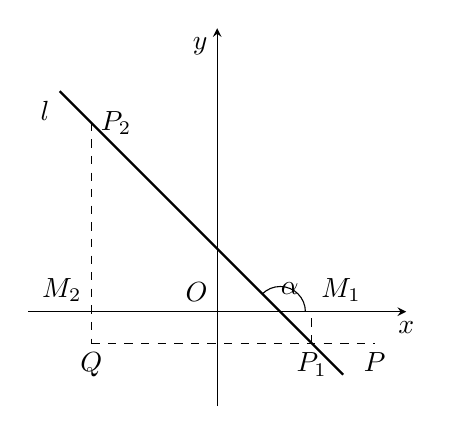
\begin{tikzpicture}[>=stealth, scale=0.8] % 箭头样式为stealth,
		% 绘制坐标轴
		\draw[->] (-3,0) -- (3,0) node[below] {$x$}; % x轴(带箭头和标签)
		\draw[->] (0,-1.5) -- (0,4.5) node[below left] {$y$}; % y轴(带箭头和标签)
		\node at (0,0) [above left] {$O$};           % 原点O的标签
		
		% 直线l  y=-x+1
		\draw[thick] (2, -1) -- (-2.5, 3.5) node[below left] {$l$}; 
		
		% 定义各关键点坐标
		\coordinate (P1) at (1.5,-0.5);  % 点P₁
		\coordinate (P2) at (-2,3); % 点P₂
		\coordinate (M1) at (1.5,0);  % 点M₁
		\coordinate (M2) at (-2,0); % 点M₂
		\coordinate (Q)  at (-2,-0.5);% 点Q
		\coordinate (P) at (2.5,-0.5);  % 点P
		
		% 绘制虚线辅助线(矩形的边)
		\draw[dashed] (Q) -- (P);  % Q到P₁的虚线
		\draw[dashed] (P1) -- (M1); % P₁到x轴的虚线
		\draw[dashed] (P2) -- (Q); % P₂到y轴的虚线
		
		% 标记各点的标签
		\node at (P) [below]  {$P$};
		\node at (P1) [below]  {$P_1$};
		\node at (P2) [right]   {$P_2$};
		\node at (M1) [above right]  {$M_1$};
		\node at (M2) [above left]  {$M_2$};
		\node at (Q)  [below]   {$Q$};
		
		%  弧线
		\draw (1.4, 0) arc (0:135:0.4) node[midway] {$\alpha$}; 
		
	\end{tikzpicture}
	
\end{document}
